\documentclass[a4paper]{report}
\usepackage[english]{babel}
\usepackage{amssymb}
\usepackage{amsmath}
\usepackage{graphicx}
\usepackage{float}
\usepackage{shortvrb}
\usepackage{cancel}
\usepackage[T1]{fontenc}
\usepackage{nicefrac}
\usepackage{amsfonts}
%nomenclature
\usepackage{makeidx}
\makeindex
\usepackage{nomencl}
\nomlabelwidth=20mm
\makenomenclature
\renewcommand{\nomname}{List of abbreviations}

\usepackage{standalone} %Makes it possible to ignore other preambles of child document
\usepackage{eurosym} %Euro teken mogelijk
\usepackage{multirow} %For multiple rows togheter in one table
\usepackage{parskip} %For a small white line between paragraphs
\usepackage[protrusion=true,expansion=true]{microtype}
\usepackage{hyperref}%For automatic and URL Reference
\usepackage[titletoc]{appendix}
%Possible to change the margins
\usepackage{geometry}
\geometry{verbose,tmargin=1.9cm,bmargin=1.7cm,lmargin=2.2cm,rmargin=2.2cm}

\usepackage{subfig}

%include pdf pages
\usepackage{pdfpages}

%Small titles
\usepackage[small,compact]{titlesec}

%being able to create tables over multiple pages
\usepackage{longtable}

\makeatletter

%Change standard font size
\renewcommand\normalsize{ \@setfontsize\normalsize{11pt}{11pt}}\normalsize  
\makeatother

\usepackage{fancyhdr}
\pagestyle{fancy}
\fancyhead{}
\fancyfoot{}

%Gives text above each page
\fancyhead[CO,CE]{DSE Project}

%Page number
\fancyfoot[RO,LE]{\thepage}


\usepackage{babel}

%Available structures:
%Report: \part{}, \chapter{}, \section{}, \subsection{}, \subsubsection{}, \paragraph{}, \subparagraph{}

\begin{document}
\chapter{Functions and Requirements of the system (5 pages, 2 text, 3 diagrams)}\label{chap:Functions}
In this chapter the the requirements for the whole system are investigated. The requirements are found using a Requirement Discovery Tree (RDT), as is explained in section \ref{sec:RDT}. Also the functions to meet this requirements are organized. The organization of the functions is done using two separate tools, the Functional Flow Diagram (FFD) and the Functional Breakdown (FB). The FB is discussed in more detail in section \ref{sec:FB}, whereas the FFD is clarified in section \ref{sec:FFD}. 

\section{Functional Breakdown}\label{sec:FB}
The Functional Breakdown is a diagram used to find all functions the product should be able to perform. These functions are performed by a combination of minor functions. By putting all minor function under the corresponding major functions, which lead to the main function to be performed by the observation platform. The FB can be seen in figure \ref{fig:FBD}.

\begin{figure}[ht]
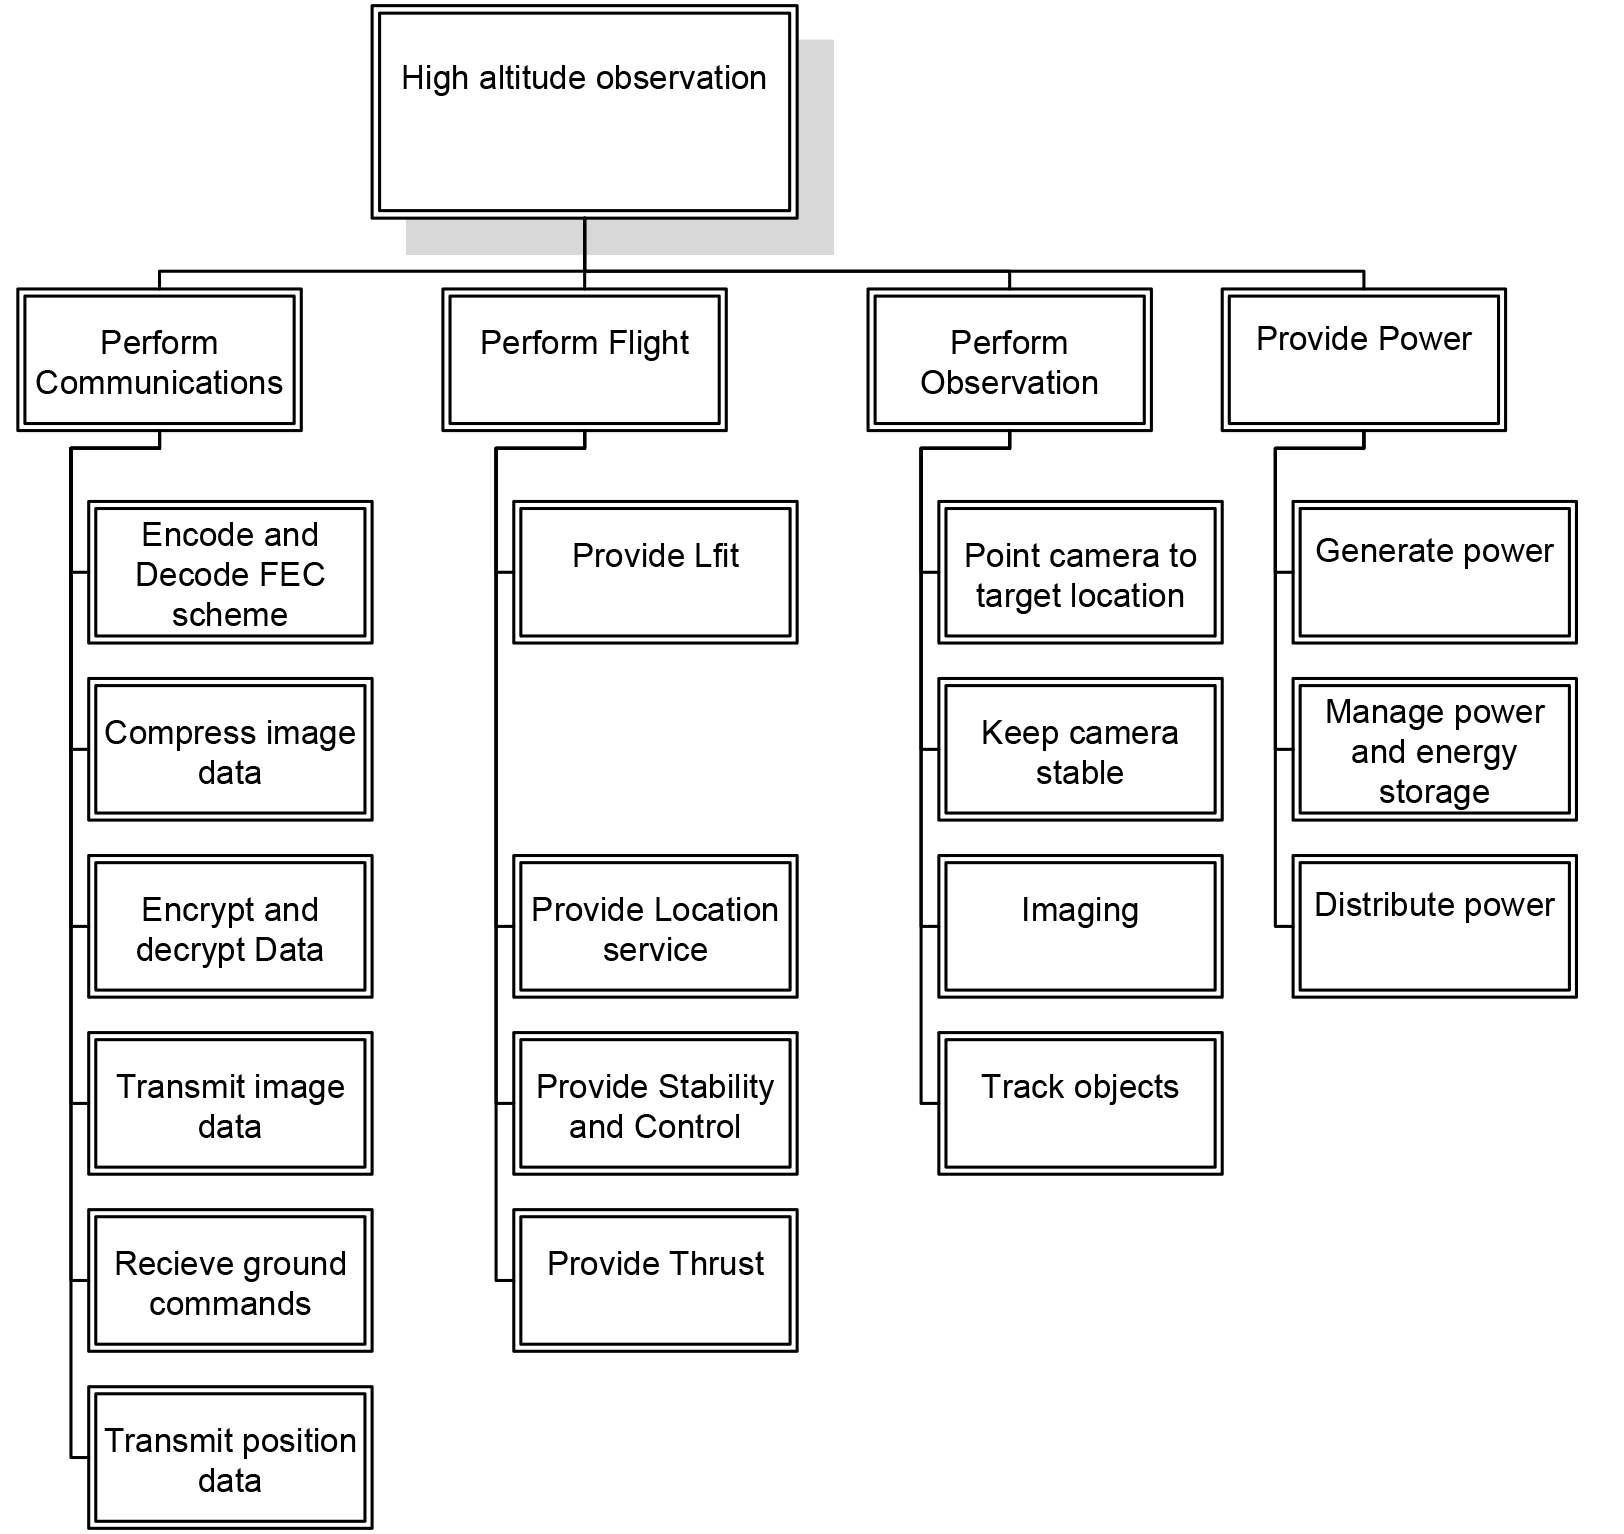
\includegraphics[width = \textwidth]{Figures/FBS/FBS.png}
\label{fig:FBD}
\caption{FBD for the all plastic high altitude observation platform}
\end{figure}

\section{Functional Flow Diagram}\label{sec:FFD}
To find the required functions for different mission elements the Functional Flow Diagram is used. The FFD shows in which order different mission segments are performed, as well as what happens per segment. The flow diagram for the mission is shown in figure \ref{fig:FFD}

\begin{figure}[ht]
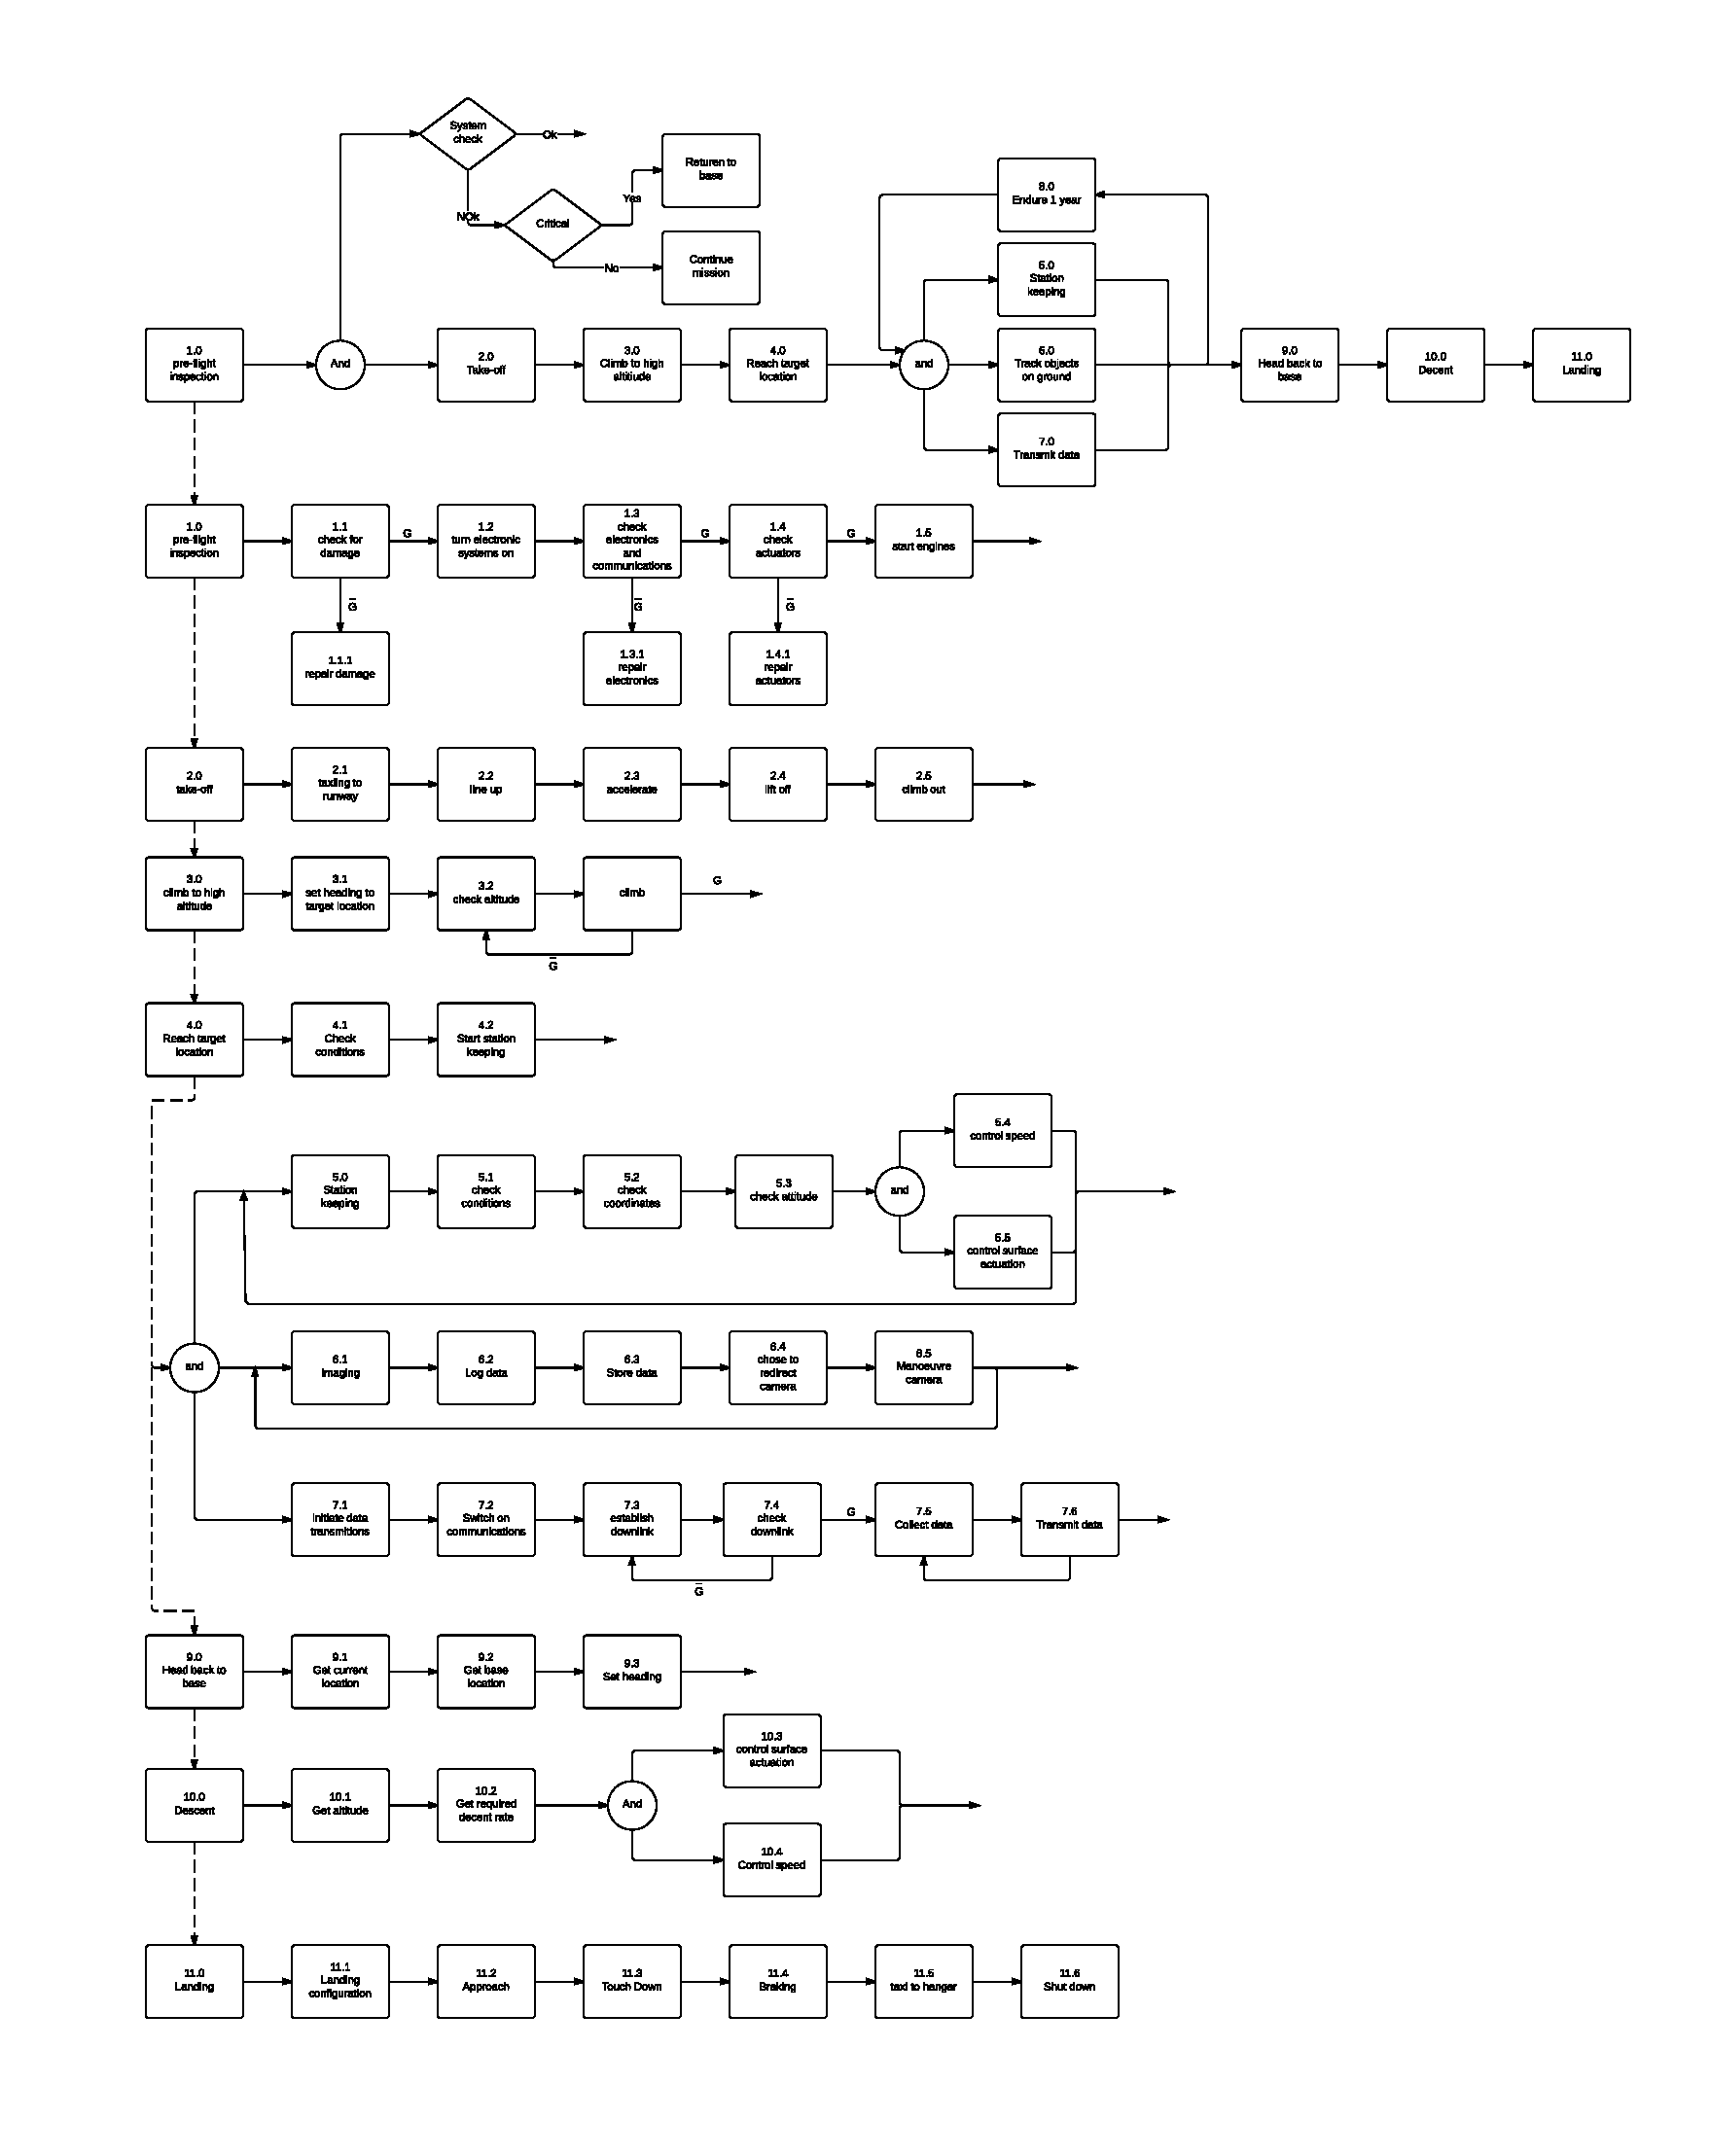
\includegraphics[width = \textwidth]{Figures/FFD.pdf}
\label{fig:FFD}
\caption{FFD for the all plastic high altitude observation platform}
\end{figure}

\section{Requirement Discovery Tree}\label{sec:RDT}
All requirements needed to fulfill the task at hand are organized in a requirement discovery tree, which can be found in figure \label{fig:RDT}. Requirements are divided in to several mission parts, which are then breaked down in more subrequirements. 

\begin{figure}
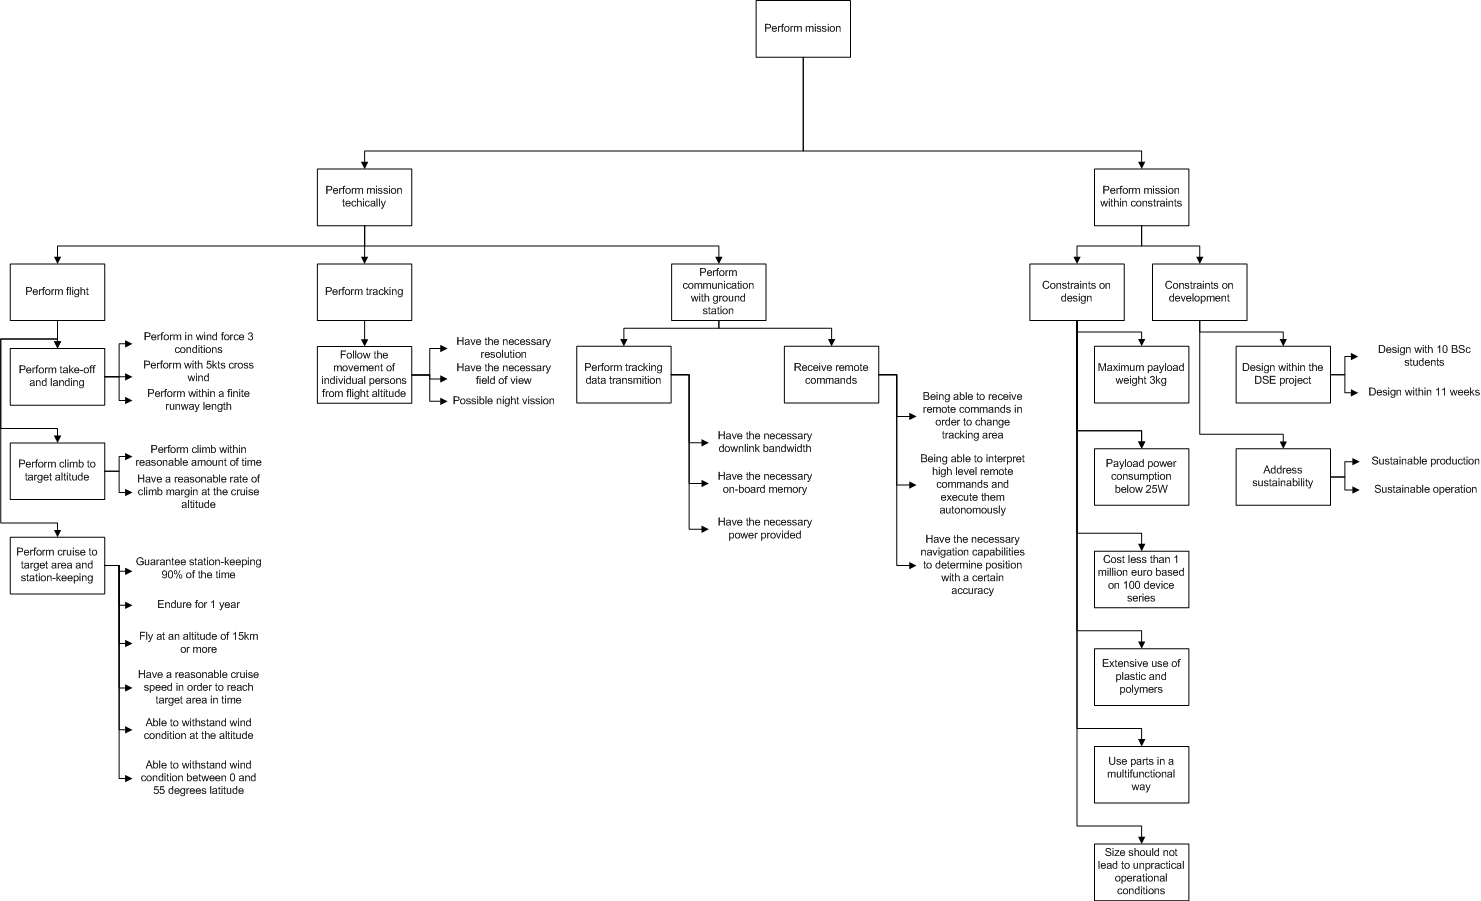
\includegraphics[width = \textwidth]{Figures/rdt.png}
\label{fig:RDT}
\caption{RDT for the all plastic high altitude observation platform}
\end{figure}

\end{document}